\documentclass{article}

\usepackage{graphicx}
\usepackage{tikz}
\usepackage{tikzsymbols}
\usetikzlibrary{calc,patterns,shapes.geometric}
\pagestyle{empty}
\usepackage[margin=0pt]{geometry}
\geometry{papersize={14in,12in}}

\def\centerarc[#1](#2)(#3:#4:#5){\draw[#1] ($(#2)+({#5*cos(#3)},{#5*sin(#3)})$) arc (#3:#4:#5);}

\begin{document}
	\begin{figure}
		\centering
		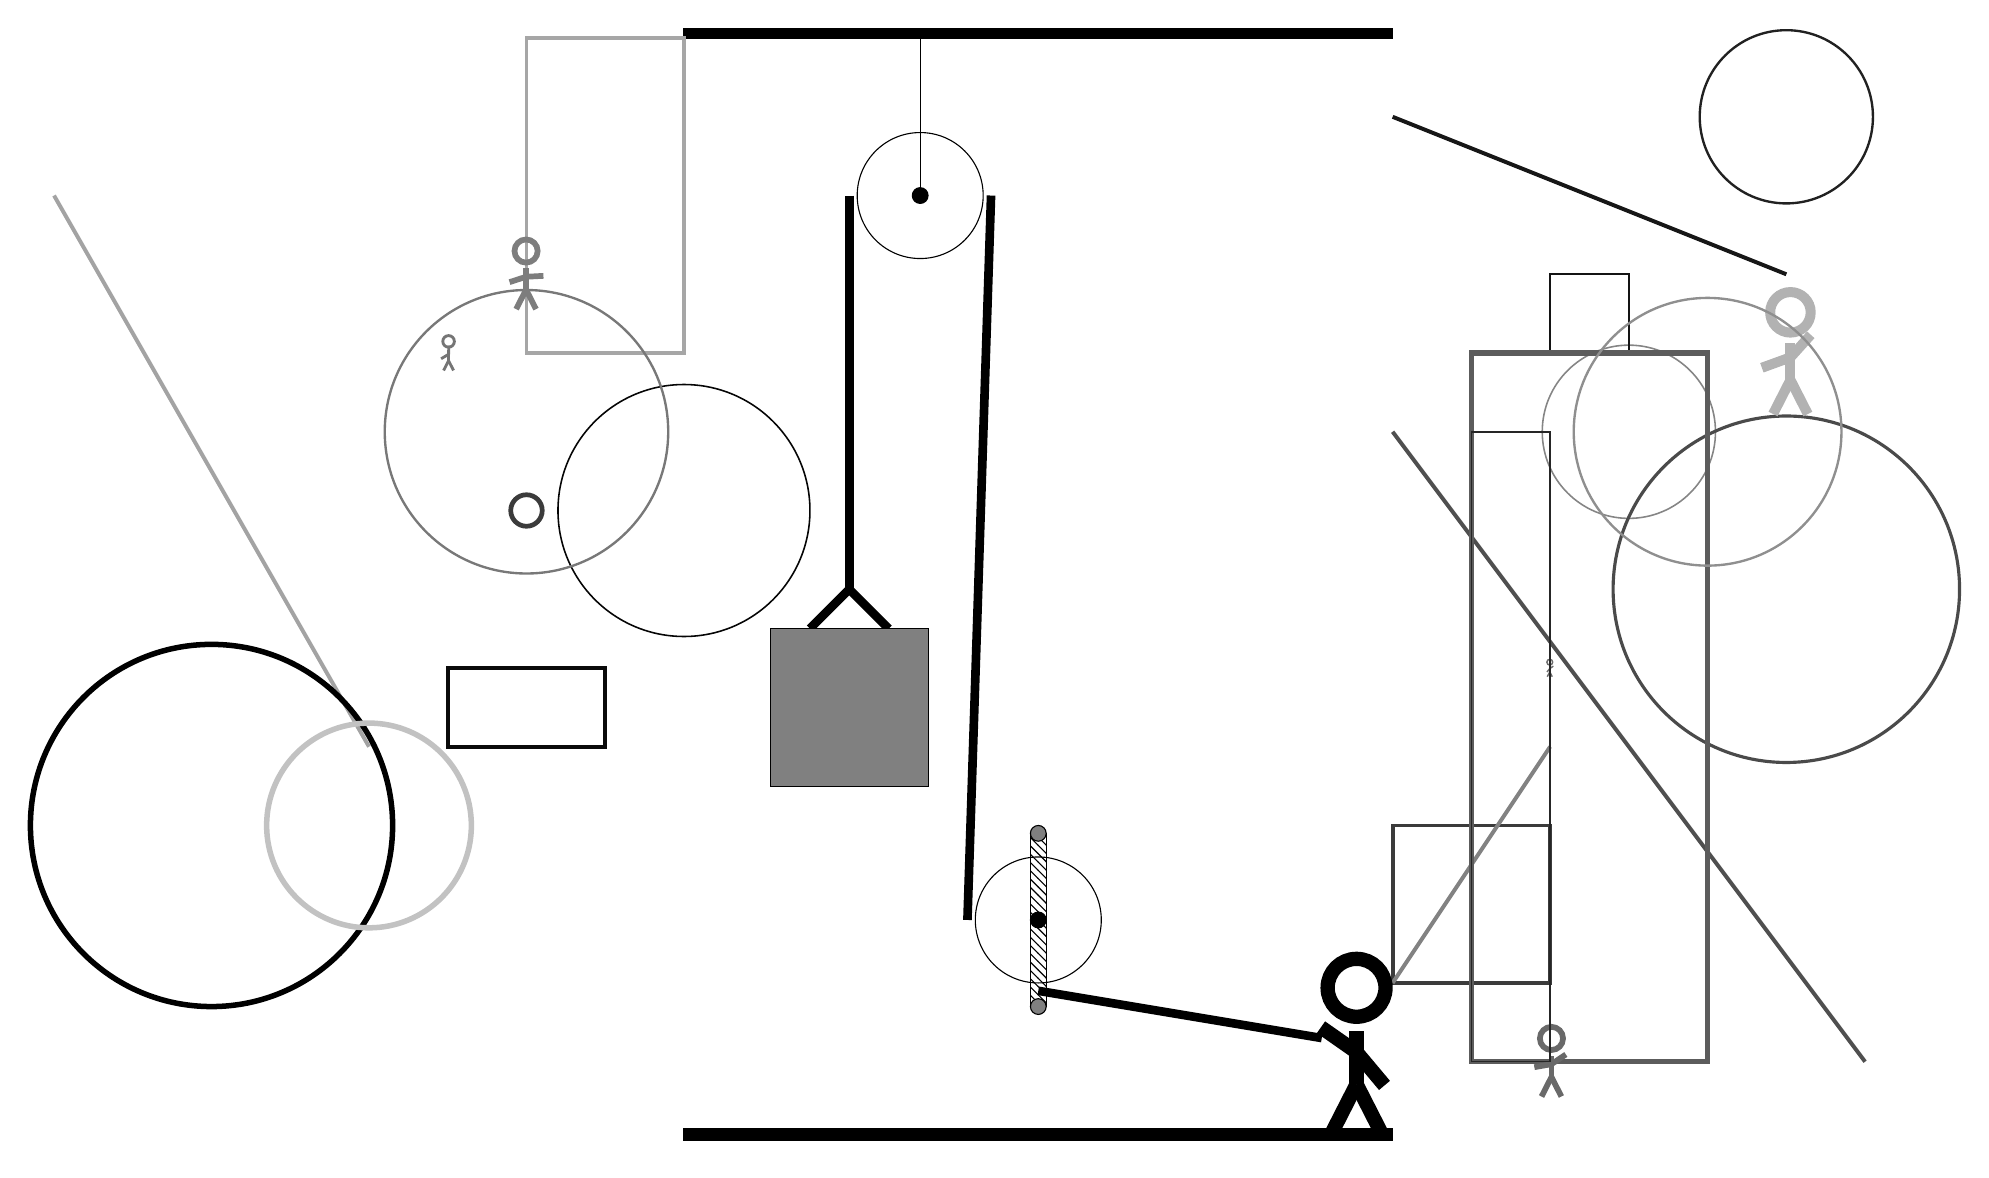
\begin{tikzpicture}
			%%%%% START %%%%%
			
			\draw[fill=black] (-2, 14) rectangle (7, 14.125);
			
			\draw (1, 12) circle (0.8);
			\draw[fill=black] (1, 12) circle (0.1);
			\draw (1, 14) -- (1, 12);
			
			\draw[fill=white](2.5, 2.8) circle (0.8);
			\draw[fill=black] (2.5, 2.8) circle (0.1);
			\draw[pattern=north west lines, pattern color=black] (2.4, 3.9) rectangle (2.6, 1.7);
			\draw[fill=black!50] (2.5, 3.9) circle (0.1);
			\draw[fill=black!50] (2.5, 1.7) circle (0.1);
			
			\draw[line width=1.1mm] (-0.4, 6.5) -- (0.1, 7.0) -- (0.6, 6.5);
			\draw[fill=black!50] (-0.9, 6.5) rectangle (1.1, 4.5);
			
			\draw[line width=0.5mm, color=black!77] (9, 4) rectangle (7, 2);
			
			\draw [line width=0.2mm, color=black!48](10, 9) circle (1.1);
			\draw [line width=0.6mm, color=black!77](-4, 8) circle (0.2);
			\draw[line width=0.5mm, color=black!91](7, 13) -- (12, 11);
			\draw[line width=0.5mm, color=black!69](7, 9) -- (13, 1);
			\draw [line width=0.2mm, color=black!98](-2, 8) circle (1.6);
			\draw [line width=0.4mm, color=black!71](12, 7) circle (2.2);
			
			\draw[line width=0.5mm, color=black!35] (-4, 14) rectangle (-2, 10);
			\node[line width=0.5mm, color=black!30] at (12, 10) {\Strichmaxerl[7][20][48]};
			
			\draw[line width=0.5mm, color=black!36](-6, 5) -- (-10, 12);
			\draw[line width=0.5mm, color=black!96] (-3, 5) rectangle (-5, 6);
			\draw [line width=0.3mm, color=black!87](12, 13) circle (1.1);
			\draw [line width=0.3mm, color=black!53](-4, 9) circle (1.8);
			
			\draw[line width=0.5mm, color=black!49](7, 2) -- (9, 5);
			\draw[line width=0.3mm, color=black!92] (9, 11) rectangle (10, 10);
			\draw[line width=0.7mm, color=black!64] (8, 10) rectangle (11, 1);
			
			\draw [line width=0.3mm, color=black!44](11, 9) circle (1.7);
			
			\node[line width=0.5mm, color=black!59] at (9, 1) {\Strichmaxerl[4][10][34]};
			\node[line width=0.3mm, color=black!58] at (9, 6) {\Strichmaxerl[1][50][35]};
			\node[line width=0.4mm, color=black!54] at (-5, 10) {\Strichmaxerl[2][31][88]};
			\node[line width=0.3mm, color=black!51] at (-4, 11) {\Strichmaxerl[4][18][3]};
			
			\draw[line width=0.2mm, color=black!85] (9, 9) rectangle (8, 1);
			\draw [line width=0.7mm, color=black!100](-8, 4) circle (2.3);
			\draw [line width=0.7mm, color=black!24](-6, 4) circle (1.3);
			
			\draw[line width=1.1mm] (0.1, 12) -- (0.1, 7.0);
			\centerarc[line width=1.1mm](1, 12)(0:180:0.9);
			\draw[line width=1.1mm](1.9, 12) -- (1.6, 2.8);
			\centerarc[line width=1.1mm](2.5, 2.8)(180:270:0.9);
			\draw[line width=1.1mm](2.5, 1.9) -- (6.1, 1.3);
			
			\node at (6.5, 1.2) {\Strichmaxerl[10][-35][-50]};
			
			\draw[fill=black] (-2, 0) rectangle (7, 0.15);
			
			%%%%% END %%%%%
		\end{tikzpicture}
	\end{figure}	
\end{document}